\subsection{本次演示采集条件与读图方法}
2026 年 10 月 26 日从正在使用的 \texttt{camera\_viewer.py} 实时演示窗口补充采集。摄像头对准实验室置物架、桌椅、纸箱及设备，维持视角和照明环境，按顺序切换板内模式和参数。所有截图均来自真实运行窗口，包含预处理按钮、阈值输入框、图像与底部状态栏；没有用 PC 算法生成灰度、二值化或边缘效果。

本次固定分辨率 $1920\times1080$、降噪强度 N32。模式与阈值对比固定 Q85；画质对比固定彩色、亮度阈值 128、边缘阈值 18。每次提交后至少等待 3 s，并确认板卡返回的实际设置与目标一致，再记录稳定窗口。模式和阈值各记录约 8 s，画质各记录约 12 s；原始采样长度、逐帧大小、板卡时间戳、状态读回和截图一并保存。

\begin{table}[H]\centering\caption{本次演示截图覆盖范围}\label{tab:livecoverage}
\small\begin{tabularx}{\linewidth}{@{}p{29mm}p{57mm}Y@{}}\toprule
类别 & 采集设置 & 固定条件\\\midrule
基础模式 & 彩色、灰度、二值化、Sobel & 1080p，N32，Q85\\
二值化阈值 & $T_b=64,96,128,160,192,224$ & 边缘阈值 18，Q85\\
边缘阈值 & $T_e=8,18,32,64$ & 亮度阈值 128，Q85\\
JPEG 画质 & Q60、Q75、Q85，末尾重复 Q60 & 彩色，N32，1080p\\\bottomrule
\end{tabularx}\end{table}

底部“JPEG fps”依据接收帧的 FPGA 时间戳统计；“显示 fps”受主机解码、缩放和窗口刷新影响。预览队列仅保留最新帧，所以“预览跳过”不等价于硬件丢帧。判断板卡链路需检查板内输入/压缩/失败 fps、编码失败、溢出和稳定窗口丢帧增量。截图中的累计准入跳帧还包含停止、启动等历史阶段，不能直接当作当前采样窗口的故障。

后续图注的带宽为独立稳定窗口平均值，截图底部是约 1 s 的即时刷新值，两者存在小幅差别。截图只改变排版尺寸，完整原图随工程提供。各参数分时采集；自动曝光、白平衡与室内光源波动未锁定，因此适合说明功能与本场景带宽变化，不能作为严格的同输入画质评价。
\evid{evidence/live_demo_summary.json；evidence/*_t*.json；images/*_window.png}
\clearpage
\subsection{彩色与灰度模式}
\begin{figure}[H]\centering
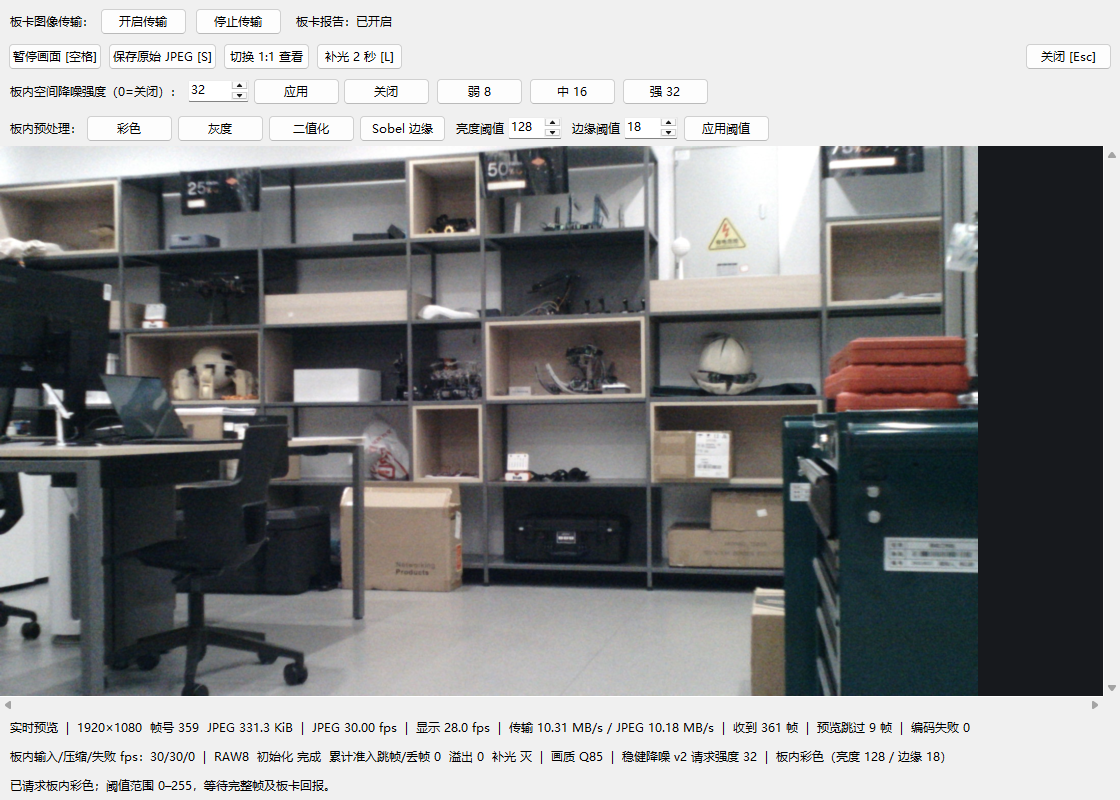
\includegraphics[width=.82\linewidth]{mode_color_window.png}
\caption{彩色模式，Q85，N32。置物架、设备和地面的颜色与亮度层次均可辨认。截图时 JPEG 331.3 KiB；稳定窗口 JPEG 载荷 10.15 MB/s、USB 接收 10.27 MB/s。}\label{fig:live-color}
\end{figure}
\begin{figure}[H]\centering
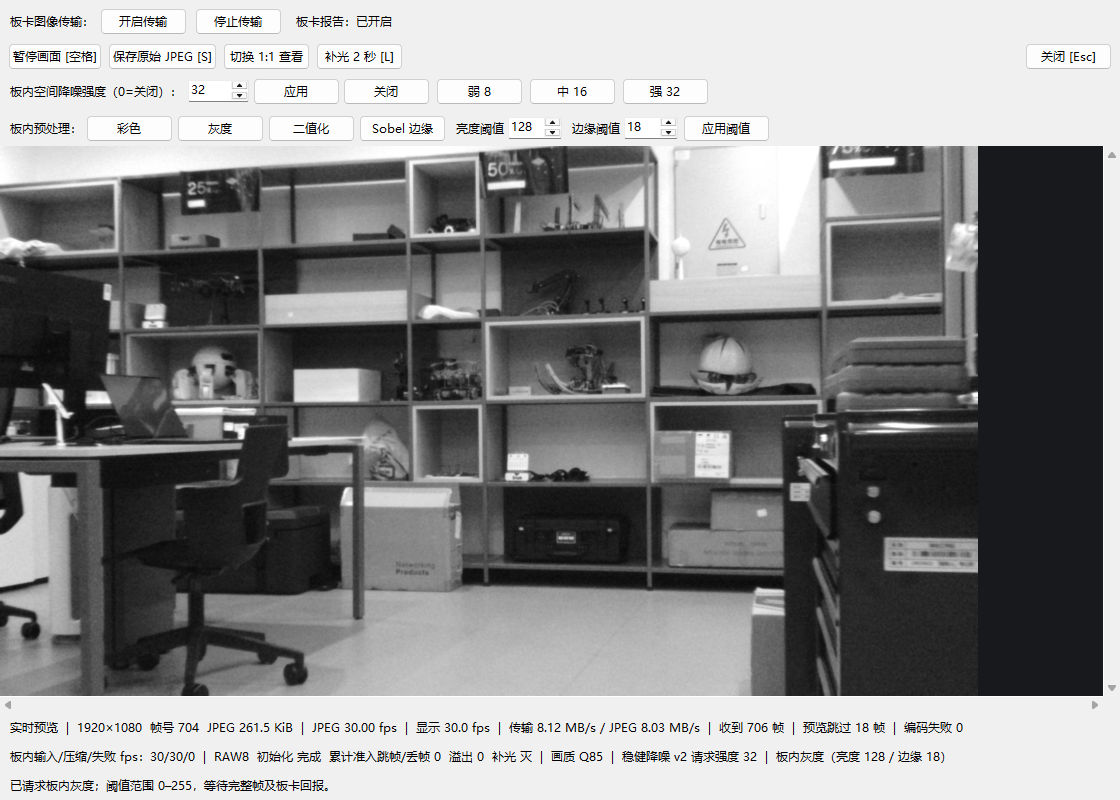
\includegraphics[width=.82\linewidth]{mode_gray_window.png}
\caption{灰度模式，Q85，N32。场景空间结构保留，色彩信息转为亮度层次。截图时 JPEG 261.5 KiB；稳定窗口 JPEG 载荷 8.05 MB/s、USB 接收 8.15 MB/s。}\label{fig:live-gray}
\end{figure}
\clearpage
\subsection{二值化阈值对比的判读}
二值化在板内比较像素亮度与阈值：$Y_{\rm out}=255$ 当 $Y\geq T_b$，否则输出 0，并将色度置为中性。提高 $T_b$ 后，只有更亮的区域保留为白色。本次选取 64～224 的六档设置，以覆盖大面积亮区、主要物体分割及高亮区域筛选。

以下各页分别显示两档真实窗口。低阈值下置物架、地面等大面积区域可能连成白块；阈值升高时较暗的隔板、设备和背景逐渐转黑，高阈值主要保留强亮区。JPEG 为有损编码，二值边界在解码后可能出现灰色过渡或轻微振铃，不能只据此判断 FPGA 比较逻辑错误。

\begin{table}[H]\centering\caption{二值化各阈值的实测载荷}\label{tab:binaryrates}
\small\begin{tabular}{@{}rrrrr@{}}\toprule
$T_b$ & 样本帧数 & 平均 JPEG (kB) & JPEG (MB/s) & USB 接收 (MB/s)\\\midrule
64 & 244 & 262.95 & 7.897 & 7.992\\
96 & 242 & 279.41 & 8.387 & 8.488\\
128 & 241 & 230.25 & 6.910 & 7.000\\
160 & 242 & 166.14 & 4.977 & 5.038\\
192 & 244 & 144.63 & 4.353 & 4.406\\
224 & 244 & 83.89 & 2.519 & 2.551\\
\bottomrule\end{tabular}\end{table}
白色面积不是码率的唯一决定因素；边界数量、形状和图像高频成分也会影响 JPEG 大小。中间阈值可能产生较复杂的明暗分界，载荷不要求随阈值单调变化。
\clearpage
\subsection{二值化阈值 64 与 96}
\begin{figure}[H]\centering
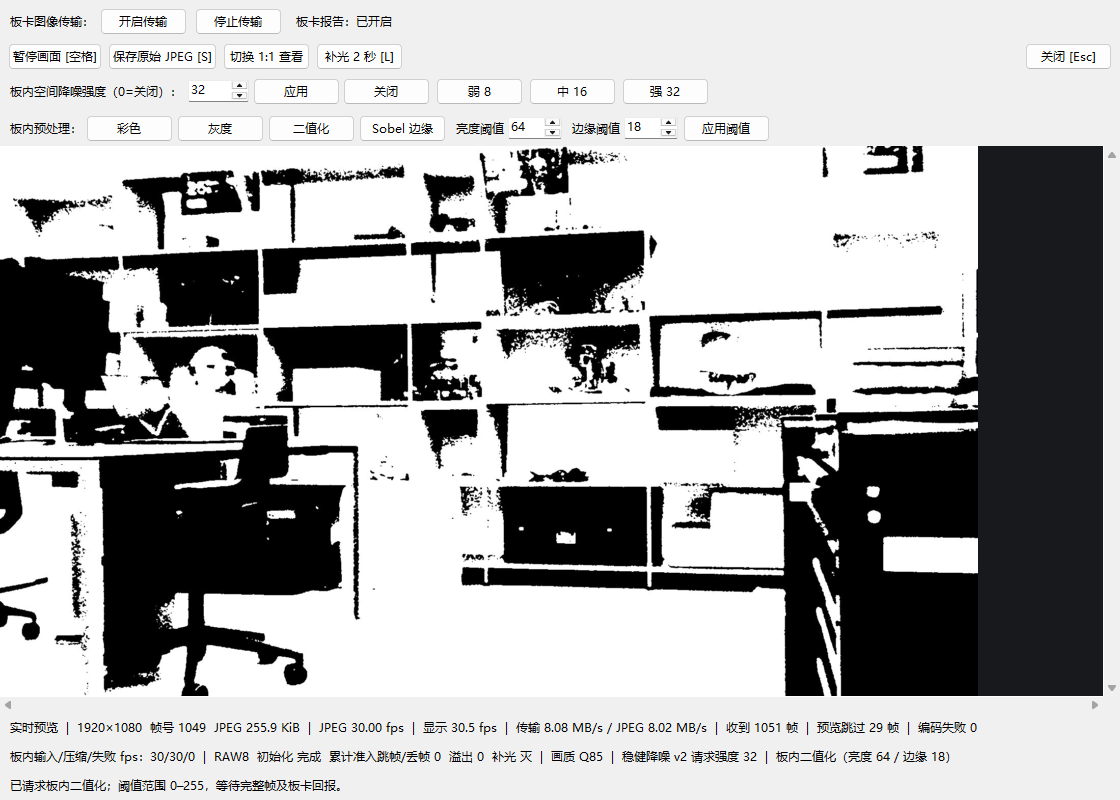
\includegraphics[width=.82\linewidth]{binary_t064_window.png}
\caption{二值化，$T_b=64$，Q85，N32。截图时 JPEG 255.9 KiB；稳定窗口 JPEG 载荷 7.90 MB/s、USB 接收 7.99 MB/s。}\label{fig:binary-64}
\end{figure}
\begin{figure}[H]\centering
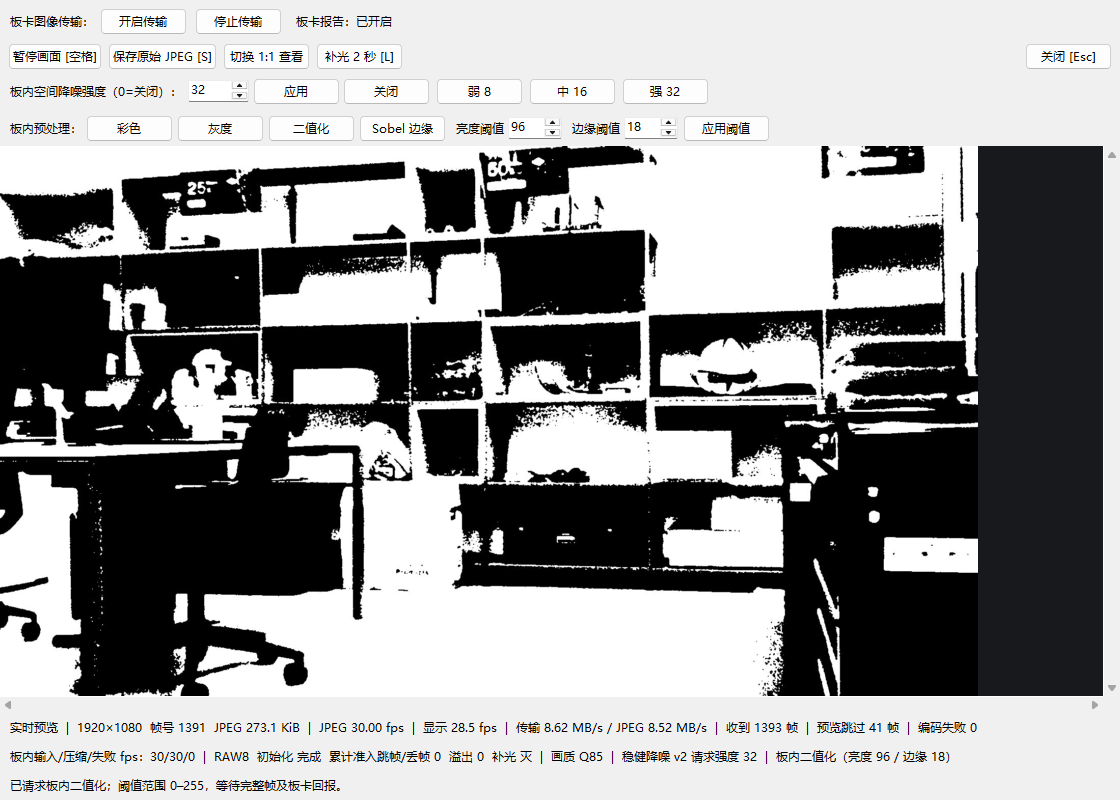
\includegraphics[width=.82\linewidth]{binary_t096_window.png}
\caption{二值化，$T_b=96$，Q85，N32。截图时 JPEG 273.1 KiB；稳定窗口 JPEG 载荷 8.39 MB/s、USB 接收 8.49 MB/s。}\label{fig:binary-96}
\end{figure}
\clearpage
\subsection{二值化阈值 128 与 160}
\begin{figure}[H]\centering
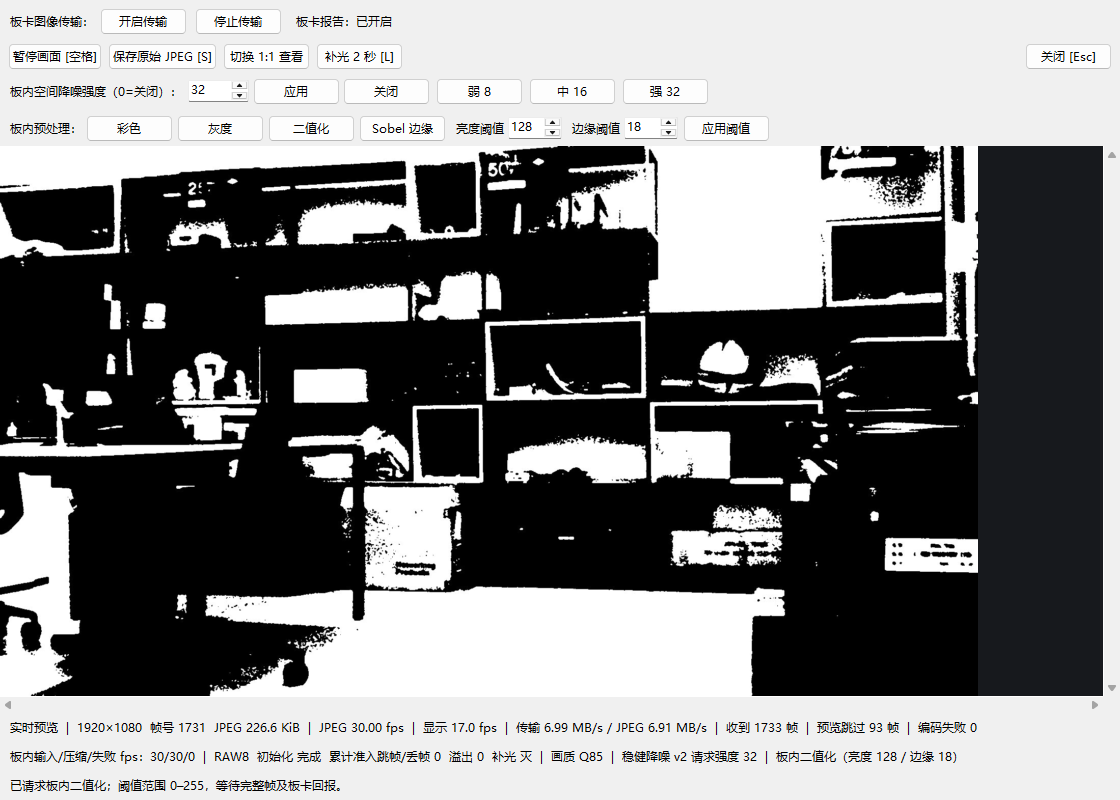
\includegraphics[width=.82\linewidth]{binary_t128_window.png}
\caption{二值化，$T_b=128$，Q85，N32。截图时 JPEG 226.6 KiB；稳定窗口 JPEG 载荷 6.91 MB/s、USB 接收 7.00 MB/s。}\label{fig:binary-128}
\end{figure}
\begin{figure}[H]\centering
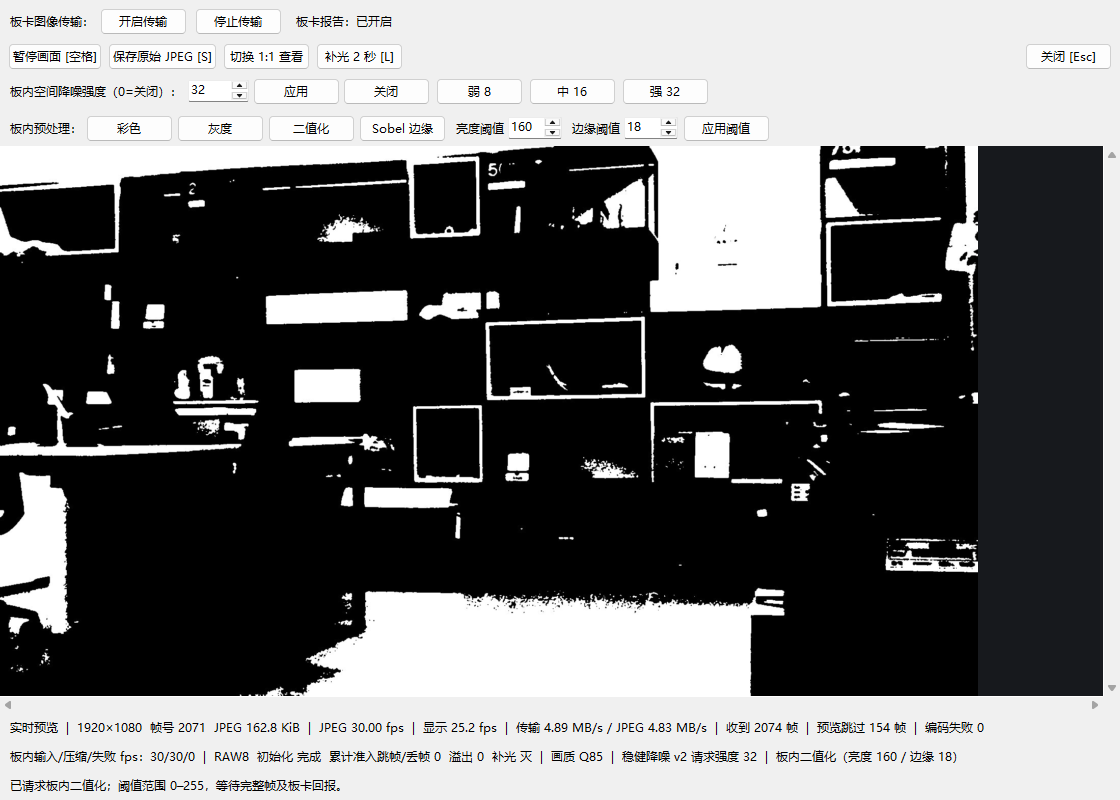
\includegraphics[width=.82\linewidth]{binary_t160_window.png}
\caption{二值化，$T_b=160$，Q85，N32。截图时 JPEG 162.8 KiB；稳定窗口 JPEG 载荷 4.98 MB/s、USB 接收 5.04 MB/s。}\label{fig:binary-160}
\end{figure}
\clearpage
\subsection{二值化阈值 192 与 224}
\begin{figure}[H]\centering
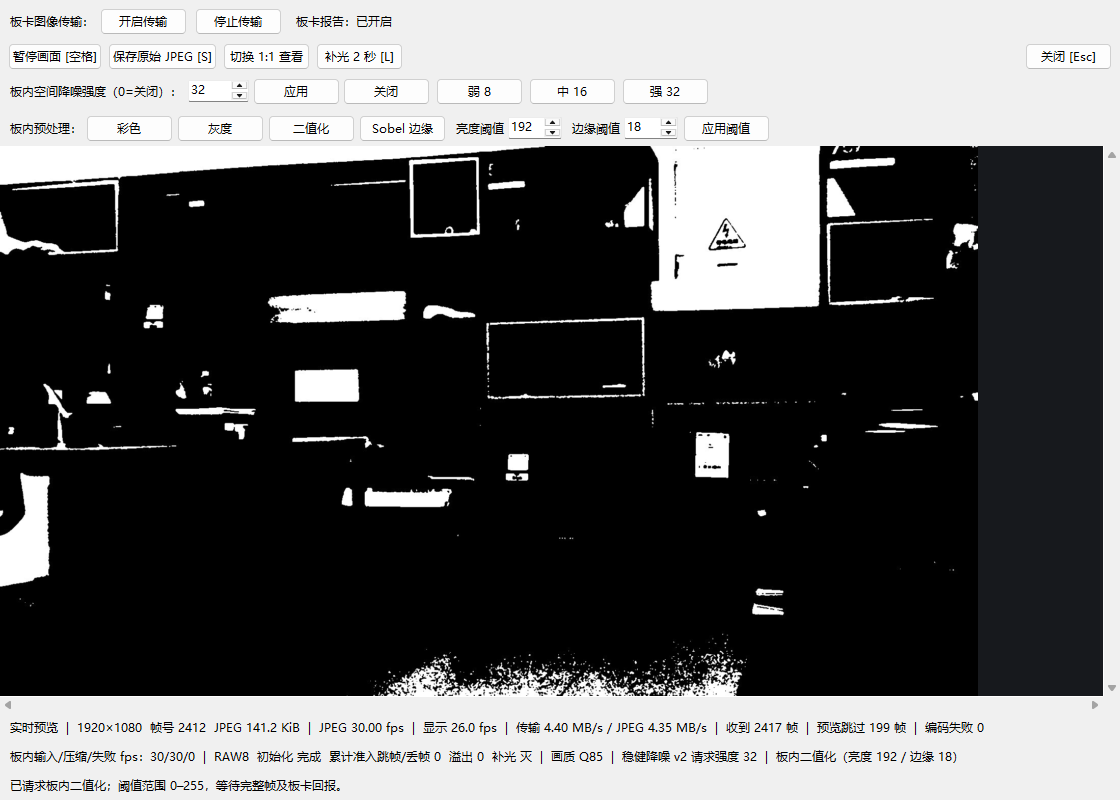
\includegraphics[width=.82\linewidth]{binary_t192_window.png}
\caption{二值化，$T_b=192$，Q85，N32。截图时 JPEG 141.2 KiB；稳定窗口 JPEG 载荷 4.35 MB/s、USB 接收 4.41 MB/s。}\label{fig:binary-192}
\end{figure}
\begin{figure}[H]\centering
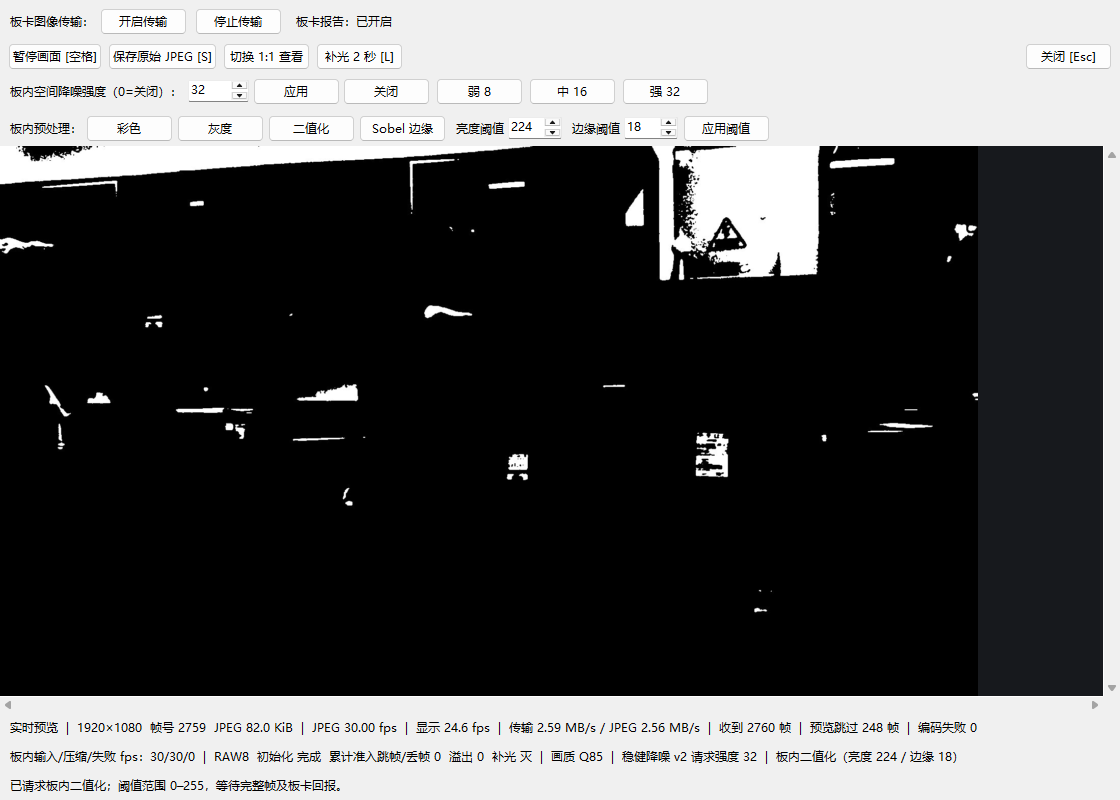
\includegraphics[width=.82\linewidth]{binary_t224_window.png}
\caption{二值化，$T_b=224$，Q85，N32。截图时 JPEG 82.0 KiB；稳定窗口 JPEG 载荷 2.52 MB/s、USB 接收 2.55 MB/s。}\label{fig:binary-224}
\end{figure}
\clearpage
\subsection{Sobel 阈值对比的判读}
当前 RTL 计算 $G_x$ 与 $G_y$ 后，使用
\[
 E=\min\!\left(255,\left\lfloor\frac{|G_x|+|G_y|+2}{4}\right\rfloor\right),
 \qquad Y_{\rm out}=\begin{cases}E,&E\geq T_e,\\0,&E<T_e.\end{cases}
\]
边缘模式保留超过阈值的梯度幅度，并不把每个边缘像素放大成纯白色。因此截图中的轮廓呈不同亮度，高阈值画面变暗也是符合实现的结果。

$T_e=8$ 能显示较多隔板、椅背、纸箱及细小纹理，但也容易保留弱变化；提高到 18、32 后，弱边缘减少；64 主要留下较强的亮度跃迁，部分连续轮廓会变细或中断。阈值应结合实际照度和目标边缘强度选择，不能只凭图像亮度高低判断检测质量。

\begin{table}[H]\centering\caption{Sobel 各阈值的实测载荷}\label{tab:edgerates}
\small\begin{tabular}{@{}rrrrr@{}}\toprule
$T_e$ & 样本帧数 & 平均 JPEG (kB) & JPEG (MB/s) & USB 接收 (MB/s)\\\midrule
8 & 240 & 293.20 & 8.778 & 8.884\\
18 & 243 & 200.69 & 6.037 & 6.101\\
32 & 244 & 173.00 & 5.184 & 5.247\\
64 & 240 & 93.24 & 2.797 & 2.832\\
\bottomrule\end{tabular}\end{table}
\src{mjpeg/rtl/camera/yuv422_preprocess.v}
\clearpage
\subsection{Sobel 边缘阈值 8 与 18}
\begin{figure}[H]\centering
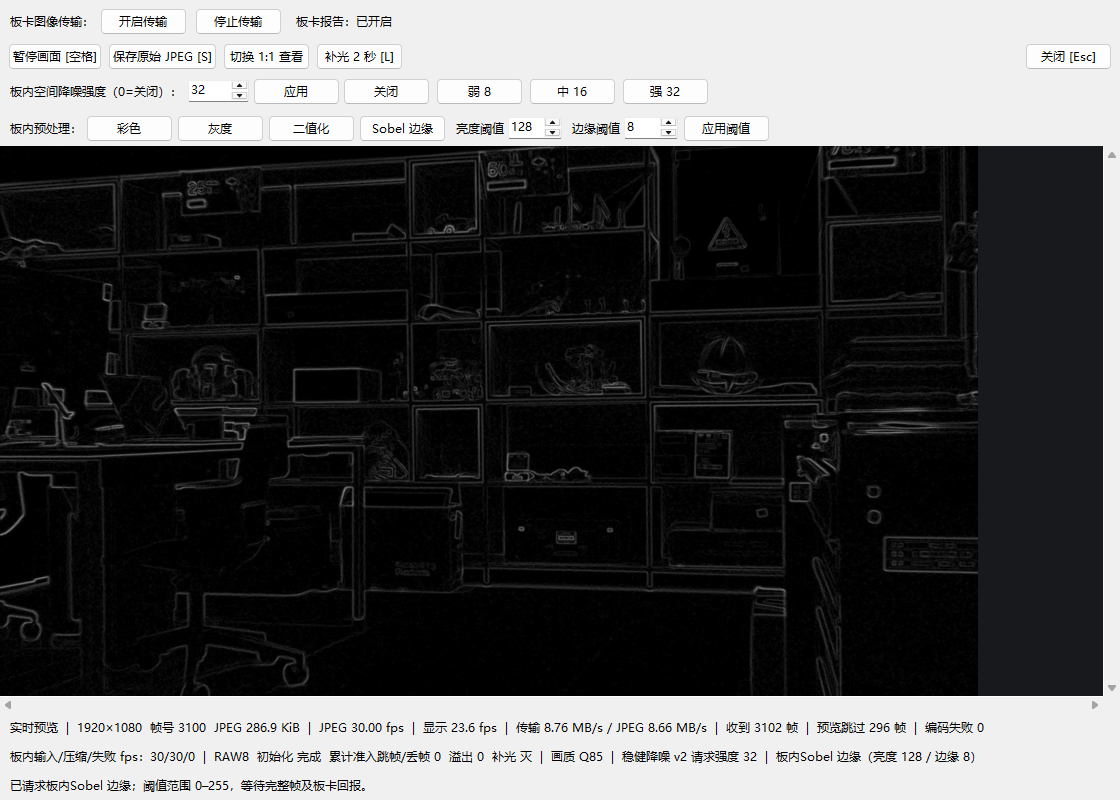
\includegraphics[width=.82\linewidth]{sobel_t008_window.png}
\caption{Sobel 边缘，$T_e=8$，Q85，N32。截图时 JPEG 286.9 KiB；稳定窗口 JPEG 载荷 8.78 MB/s、USB 接收 8.88 MB/s。}\label{fig:edge-8}
\end{figure}
\begin{figure}[H]\centering
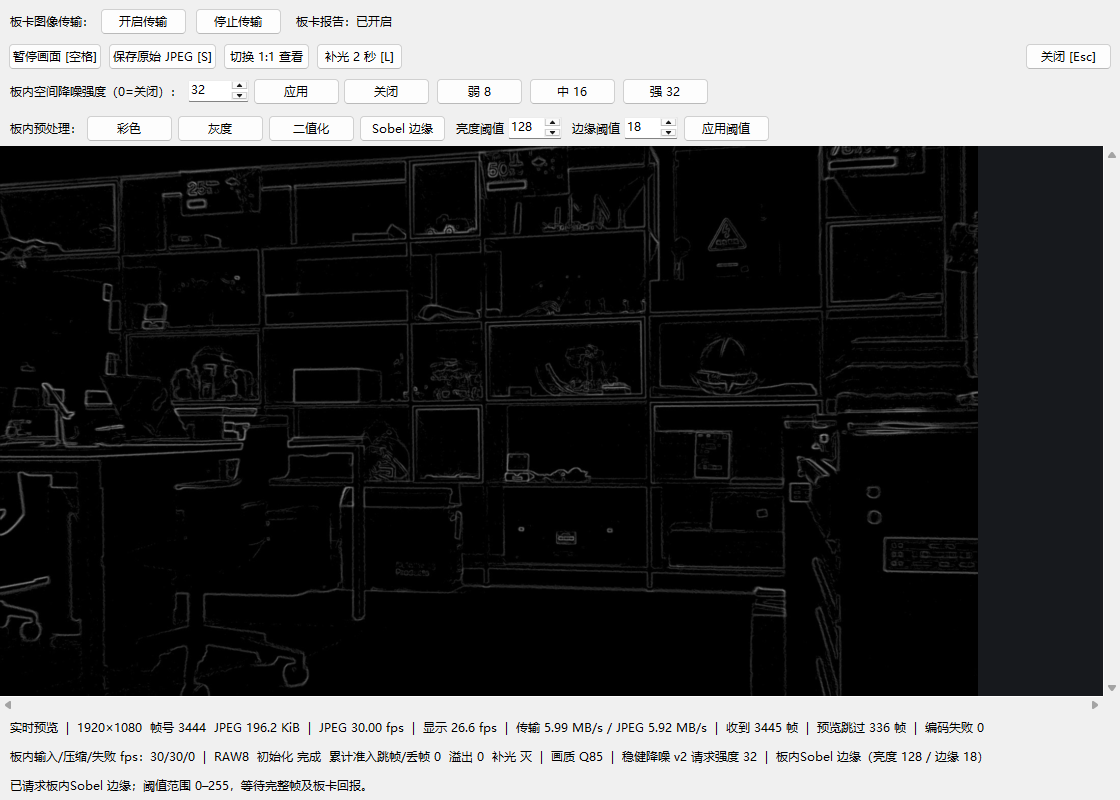
\includegraphics[width=.82\linewidth]{sobel_t018_window.png}
\caption{Sobel 边缘，$T_e=18$，Q85，N32。截图时 JPEG 196.2 KiB；稳定窗口 JPEG 载荷 6.04 MB/s、USB 接收 6.10 MB/s。}\label{fig:edge-18}
\end{figure}
\clearpage
\subsection{Sobel 边缘阈值 32 与 64}
\begin{figure}[H]\centering
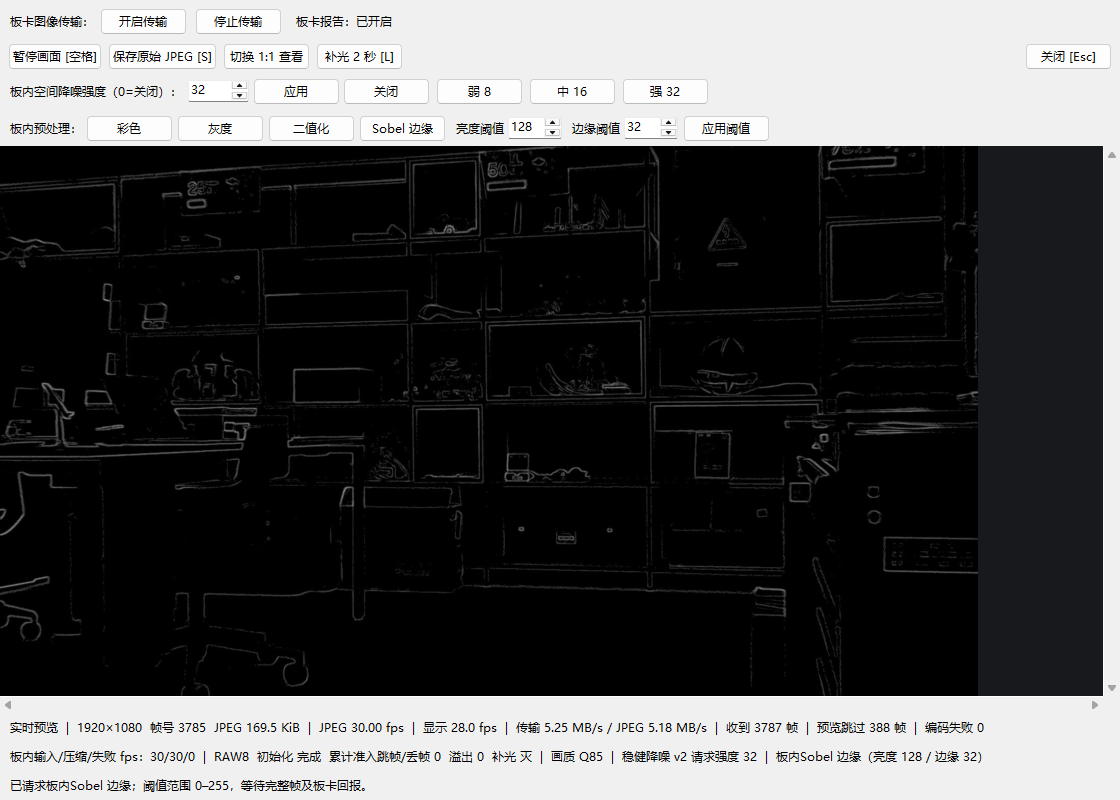
\includegraphics[width=.82\linewidth]{sobel_t032_window.png}
\caption{Sobel 边缘，$T_e=32$，Q85，N32。截图时 JPEG 169.5 KiB；稳定窗口 JPEG 载荷 5.18 MB/s、USB 接收 5.25 MB/s。}\label{fig:edge-32}
\end{figure}
\begin{figure}[H]\centering
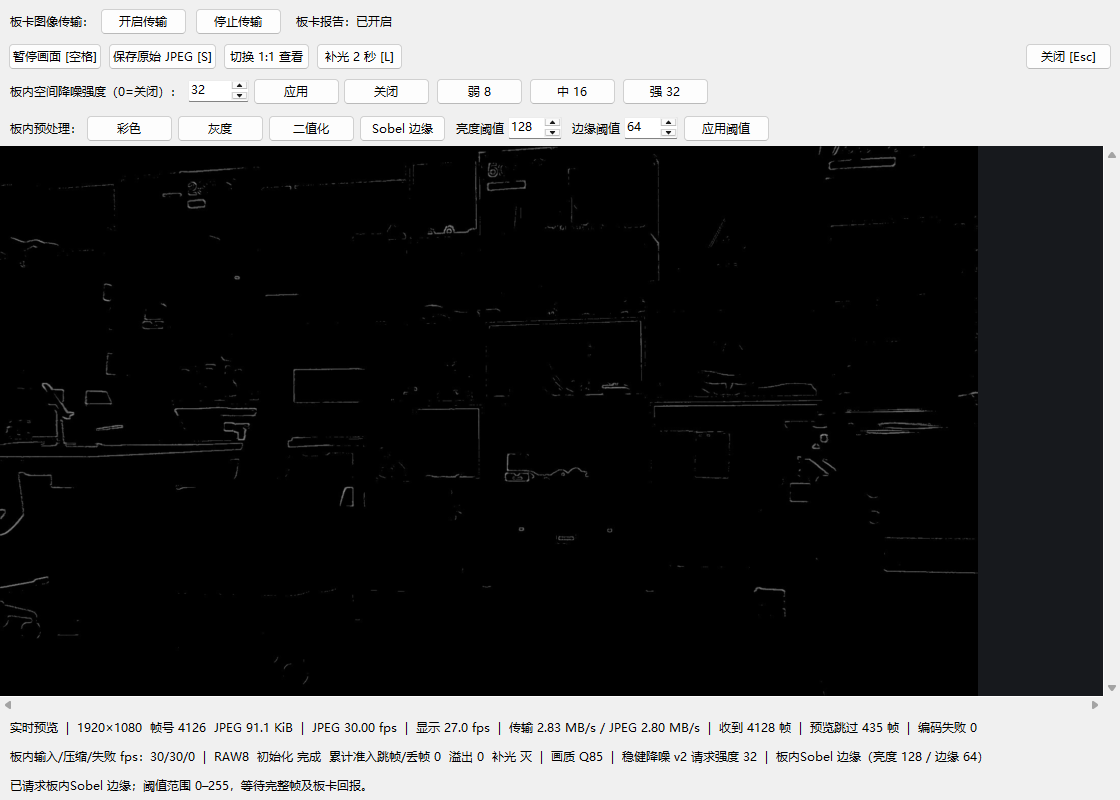
\includegraphics[width=.82\linewidth]{sobel_t064_window.png}
\caption{Sobel 边缘，$T_e=64$，Q85，N32。截图时 JPEG 91.1 KiB；稳定窗口 JPEG 载荷 2.80 MB/s、USB 接收 2.83 MB/s。}\label{fig:edge-64}
\end{figure}
\clearpage
